\chapter{Technical Indicator based Backtesting}
\label{chap:technical_backtesting}


\section{Input Data}

All the cryptocurrency historical data used in this project was downloaded using the \texttt{data\_retriever} module, which establishes a connection with the Binance server
and fetches data for defined crypto symbols (a crypto symbol represents a specific cryptocurrency,
like BTC for Bitcoin or ETH for Ethereum) over a specified period.
The downloaded data is stored in the \texttt{historical\_data} directory. Each symbol has its own directory, where the corresponding data is
saved in a \texttt{.parquet.gzip} format.
Data is downloaded at a one-minute frequency but can be downsampled to longer intervals, such as 1 hour or 1 day.

The \texttt{load\_data.py} module facilitates loading the historical data of a symbol from its \texttt{.parquet.gzip} file for use in backtesting strategies.

\begin{figure}[h]
\dirtree{%
.1 backtester.
.2 historical\_data.
.3 BTCUSDT.
.4 BTCUSDT.parquet.gzip.
.3 ETHUSDT.
.4 ETHUSDT.parquet.gzip.
.3 \ldots.
.2 \ldots.
.2 utilities.
.3 data\_utils.
.4 data\_loader.py.
.4 data\_retriever.py.
.4 ml\_data\_manager.py.
.4 ml\_feature\_engineer.py.
}

\caption{Data-centric modules and folders.}\label{fig:inputdata}
\end{figure}

\section{Technical Indicator-based Strategies}
Technical indicators are statistical calculations based on historical price and volume information that aim to predict future price movements.
Commonly used in technical analysis, these indicators provide insight into the market's direction, strength, momentum, and volatility.
The backtesting architecture, including the necessary classes and components for strategies based on technical indicators is depicted in UML diagram~\ref{fig:tech_indicator_arch}.
One of the main advantages of the framework is its extensibility. It allows the integration and configuration of new strategies.
To integrate a new algorithm, it should inherit from the \texttt{BacktesterBase} class found in the \texttt{backtester\_base.py} module. Additionally, it must implement the following methods: \texttt{prepare\_data}, \texttt{optimize\_strategy}, \texttt{objective()}, and \texttt{test\_strategy()}.
Figure~\ref{fig:tech_indicator_arch} showcases the framework's architecture specifically for technical indicator-based backtesting.
The \texttt{MacdBacktester} class (highlighted in red) inherits common attributes and methods from the \texttt{BacktesterBase} class,
such as \texttt{get\_data}, \texttt{run\_backtest}, \texttt{add\_stop\_loss}, and \texttt{add\_take\_profit}, among others.

\begin{figure}[ht!]
\centering
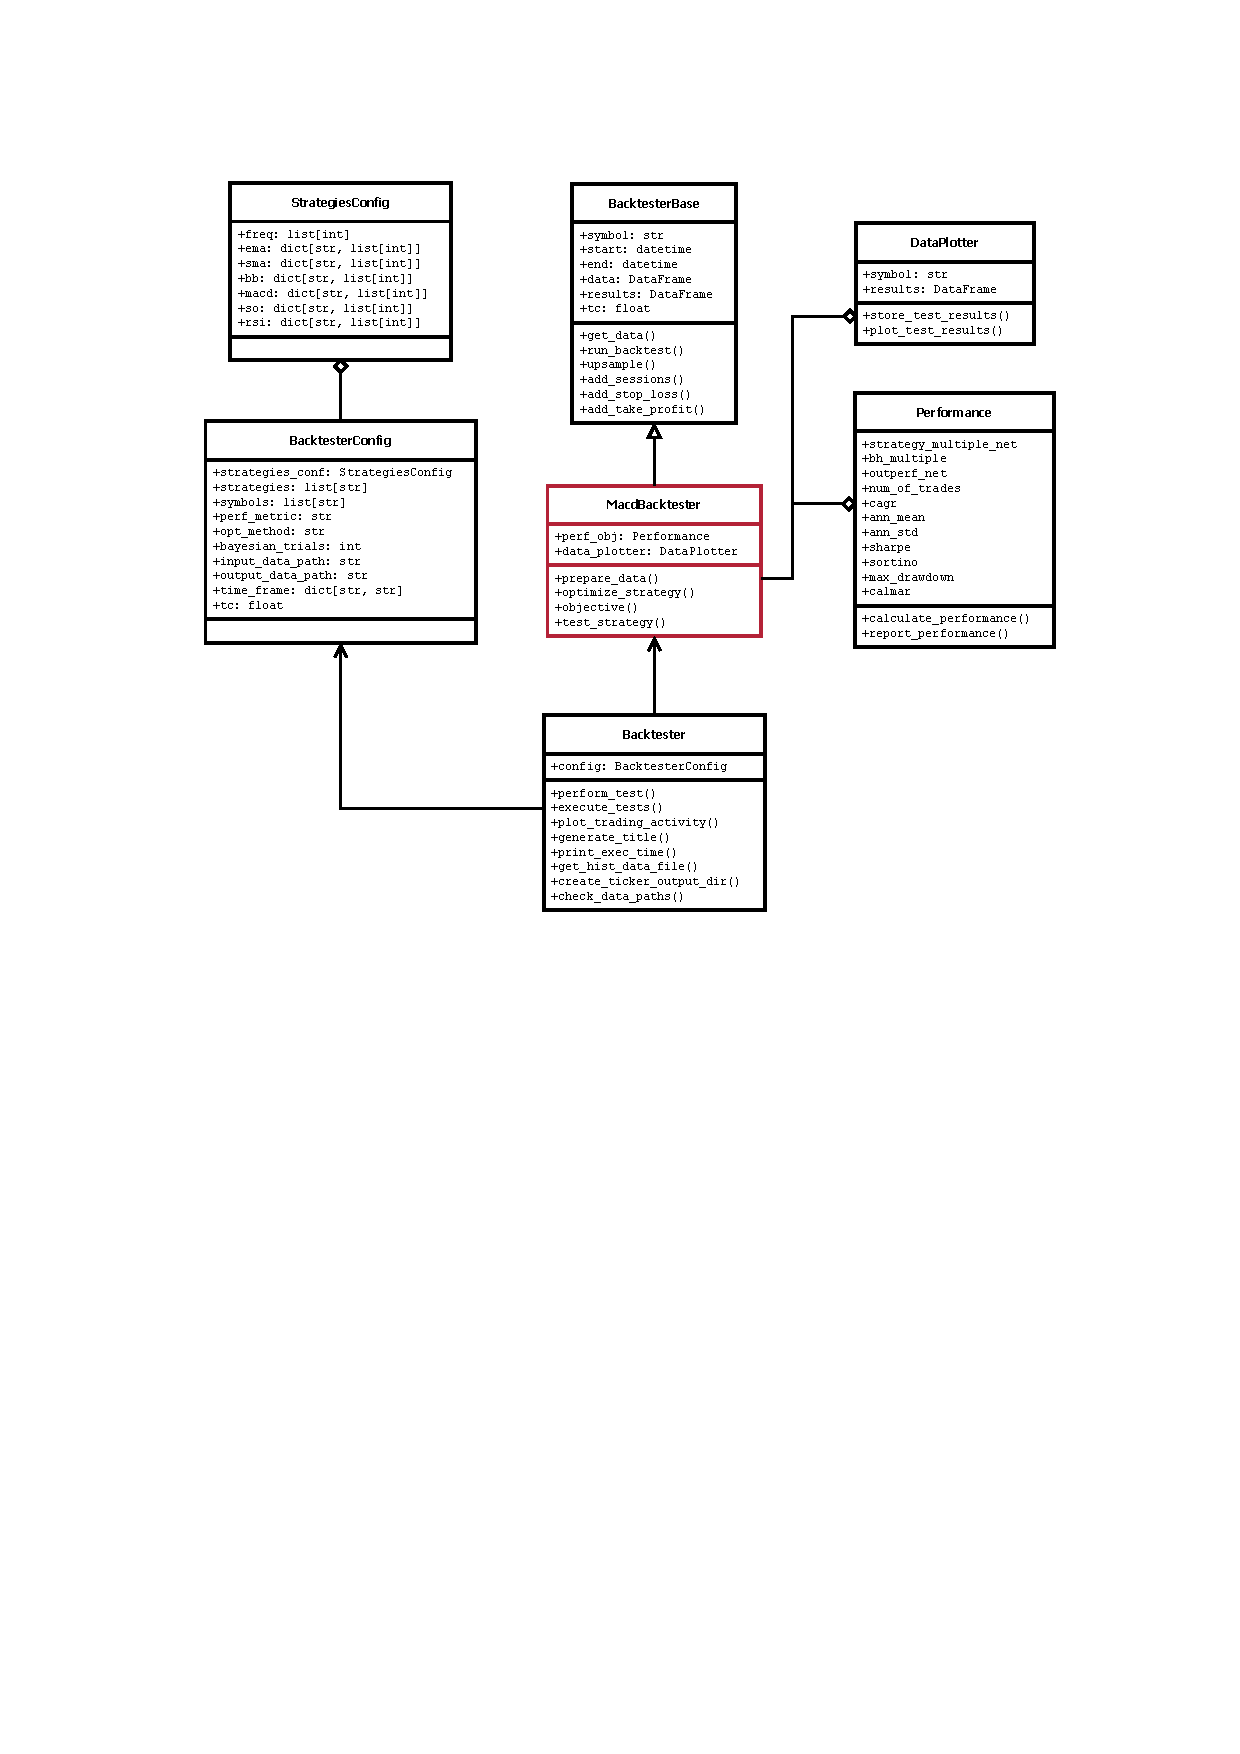
\includegraphics[page=1, trim=30mm 135mm 0 25mm, width=1.1\textwidth, clip]{./pdf/backtester_uml.pdf}
\caption{Technical indicator based backtesting architecture.}
\label{fig:tech_indicator_arch}
\end{figure}

The \texttt{DataPlotter} and \texttt{Performance} classes are utilized to compute and visually display performance metrics for each test run.
The \texttt{Backtester} class manages the entire backtesting process, leveraging the functionalities of other classes to perform its tasks.
The \texttt{BacktesterConfig} class represents the configuration, which is validated and ingested in the \texttt{Backtester} class via the Python \texttt{pydantic} library.

For optimization, either the grid search method or the Bayesian method can be chosen. The former comprehensively explores all possible combinations in the parameter ranges,
while the latter utilizes probability distributions to refine its search. Depending on the defined parameter ranges for each algorithm, a vast array of combinations, potentially
in the tens of thousands, can be assessed for each symbol. Performance results for all these tests are saved into a dedicated \texttt{\{symbol\}.csv} file
located in the \texttt{results/\{symbol\}} directory, facilitating subsequent analysis and visualizations.


The Listing~\ref{lst:ml_config} shows how the Backtester is set up to run backtests for XRP, LTC, and TRX with an EMA-based strategy.
The Bayesian method is used for optimization, and EMA parameter ranges are defined. Each symbol's results will be stored in its respective .csv file.

\begin{lstlisting}[style=jsonstyle, caption={Machine Learning Pipeline Configuration},  label=lst:ml_config]
{
  "opt_method": "bayesian",
  "bayesian_trials": 1500,
  "time_frame": {
    "start_date": "",
    "end_date": "2022-12-31 23:59:00"
  },
  "symbols": ["XRPUSDT", "LTCUSDT", "TRXUSDT"],
  "strategies_config":
  {
    "freq" : [5, 125, 5],
    "ema": {
       "ema_s": [6, 60, 4],
       "ema_l": [10, 200, 5]
    }
  }
}
\end{lstlisting}

Furthermore, individual backtesting results for each symbol and applied strategy can be visualized,
as shown in fig.~\ref{fig:backtest_results}. This figure displays the effectiveness of the optimized strategy
compared to the buy-and-hold approach. As an example, the \texttt{EMA} strategy was used for the \texttt{LTCUSDT} symbol. All pertinent parameters are
illustrated above the primary plot. Testing was executed on historical data ranging
from 2021-01-01 to 2021-12-31.

\begin{figure} [H]
\centering
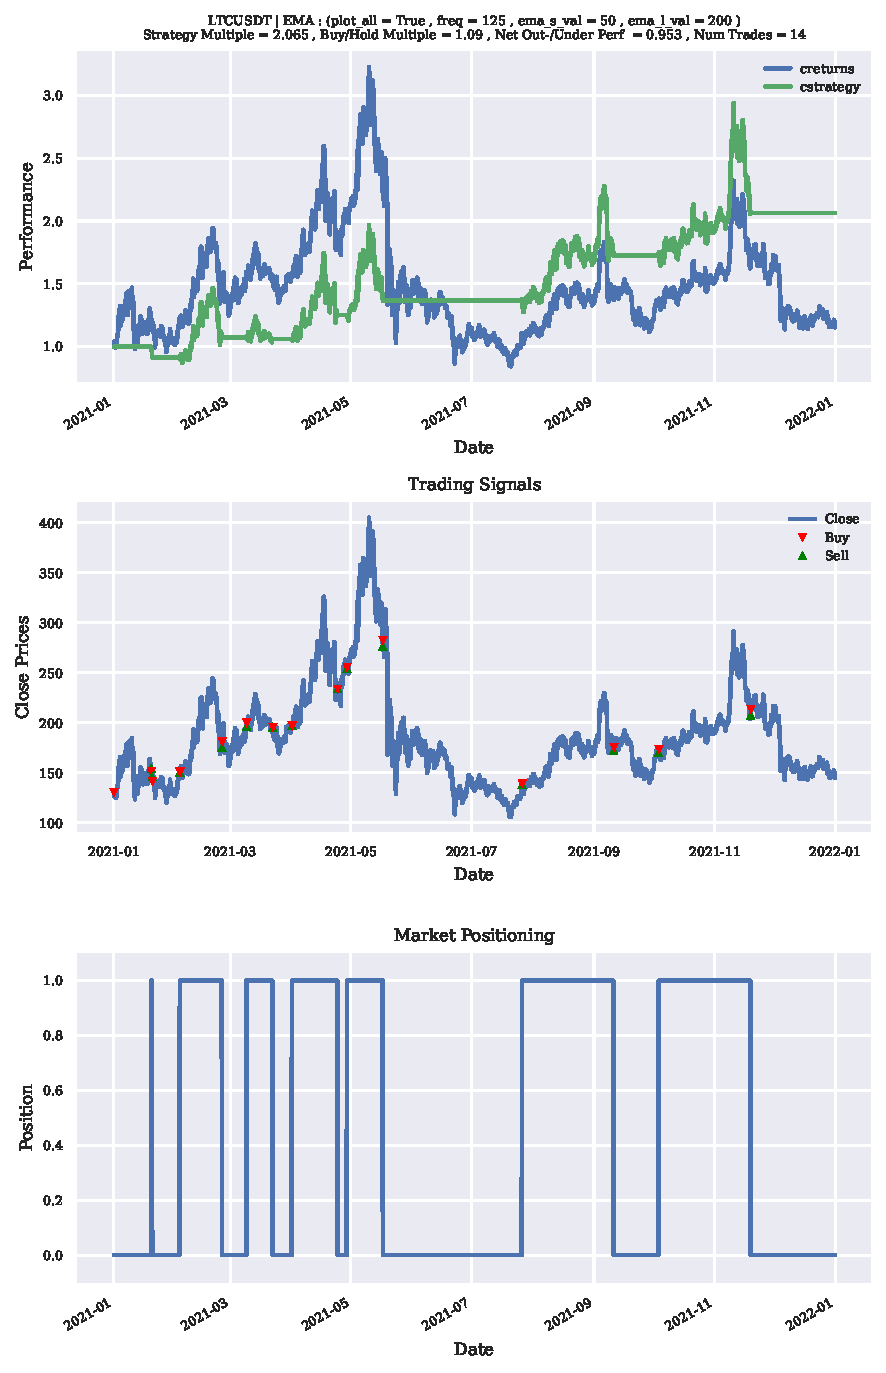
\includegraphics[page=1, trim=0mm 0mm 0 0mm, width=0.95\textwidth, clip]{./pdf/backtesting_results.pdf}
\caption{Results of Backtesting of MACD Stragegy of XRPUSDT.}
\label{fig:backtest_results}
\end{figure}

The secondary plot, demonstrates the close prices of LTCUSDT,
marked with buy (red triangle) and sell (green triangle) signals generated by the EMA strategy.
The bottom plot, "Market Positioning", illustrates the duration of each position, with 1 indicating a long position and 0 no position.

\begin{table}[H]
    \centering
    \begin{tabular}{l}
        \texttt{LTCUSDT | EMA : (freq = 125 , ema\_s\_val = 50 , ema\_l\_val = 200)} \\
        \texttt{Strategy Multiple = 2.065 , Buy/Hold Multiple = 1.09} \\
        \texttt{Net Out-/Under Perf = 0.953 , Num Trades = 14} \\
    \end{tabular}
    \caption{Backtesting results and parameters for the EMA strategy on LTCUSDT .}
    \label{tab:backtest_results}
\end{table}

Table~\ref{tab:backtest_results} provides a detailed overview of the parameters used for the EMA strategy, such as frequencies, long and short window periods as well as performance metrics.
The strategy  performed quite well and outperformed the buy-and-hold benchmark, achieving an outperformance of a 95\%.
% trim={<left> <lower> <right> <upper>}
%\vspace{-2cm}


%Parameters:
%{'algorithm': 'SAMME', 'base_estimator': None, 'learning_rate': 0.5, 'n_estimators': 100, 'random_state': None}







